\documentclass[10pt]{article}
\usepackage[margin=1in]{geometry}
\usepackage{amsmath,amssymb,amsthm}
\usepackage{graphicx}
\usepackage{booktabs}
\usepackage{hyperref}
\usepackage{xcolor}
\usepackage[numbers,sort&compress]{natbib}
\usepackage{subcaption}
\usepackage{multirow}
\usepackage{longtable}
\usepackage{lineno}
\usepackage{setspace}
\graphicspath{{figures/}}

\newtheorem{proposition}{Proposition}
\newtheorem{corollary}[proposition]{Corollary}

\newcommand{\citeneeded}[1]{\textcolor{red}{[CITE: #1]}}
\newcommand{\todo}[1]{\textcolor{orange}{[TODO: #1]}}

\title{Higher-order knockout epistasis is generated by dynamics, not molecular wiring, in 27 Boolean gene regulatory networks}

\author{
  Elliot Tower\textsuperscript{1,2,*} \\[4pt]
  \small\textsuperscript{1}Mechanistic Research \\
  \small\textsuperscript{2}University of Edinburgh \\
  \small\textsuperscript{*}Correspondence: \texttt{elliot@mechanisticresearch.org}
}

\begin{document}
\maketitle
\linenumbers
\doublespacing

\begin{abstract}
Nonlinear dynamics generate pairwise statistical epistasis from
molecular architectures that need not contain epistatic terms
\citep{gjuvsland2007statistical}; whether this extends to
higher-order interactions, and with what magnitude and sign, has not
been quantified. Each gene's regulatory logic involves a few direct
partners; knockout phenotypes reflect the full composed dynamics.
Across 27 published Boolean network models (7--17 genes), exhaustive
$2^n$ combinatorial knockout sweeps reveal a systematic composition
gap between the interaction spectra of individual gene rules and the
attractor-level knockout phenotype. A Walsh--Hadamard decomposition
---which partitions phenotypic variance into contributions from
single genes, gene pairs, triplets, and higher-order
combinations---shows that dynamics create higher-order interactions
in 18 of 24 non-null networks ($|\Delta_{3+}| \geq 0.5$~pp), with
gaps from $< 1$ to $+83$ percentage points of higher-order spectral
energy. In five networks, molecular wiring fails to predict knockout
epistasis---gene pairs with the strongest local interactions show the
weakest global effects. Pre-registered structural predictions
(feedback loop counts, rule complexity, in-degree distribution) on 21
held-out networks achieve 48\% direction accuracy, indistinguishable
from chance. Hill-function ODE conversion preserves the gap sign in
all 22 networks tested. Separately, three experimental fitness
landscapes show higher-order epistasis beyond additive expectations
in real organisms, confirming that higher-order structure exists
though this tests an additive baseline rather than the local-rule
comparison of the Boolean analysis. Creation dominance is specific to
loss-of-function knockouts: gain-of-function clamping reverses the
ratio. These results suggest that predicting higher-order knockout
epistasis will require models of the composed dynamics rather than
molecular interaction data alone.
\end{abstract}

\noindent\textbf{Keywords:}
epistasis, Boolean networks, gene regulatory networks,
Walsh--Hadamard transform, composition gap, knockout screens


\section*{Author summary}
Genes rarely act alone: knocking out multiple genes often produces
effects that no single knockout predicts. Biologists call this epistasis.
The molecular wiring of a gene regulatory network specifies pairwise
interactions, but the phenotype depends on the long-run dynamics of the
entire network. We ask: does dynamical composition systematically create
or destroy higher-order epistasis? Across 27 published Boolean network
models, we find that dynamics create higher-order interactions three
times more often than they destroy them. The molecular wiring diagram
provides some guidance---local interaction strength correlates with
knockout epistasis in most networks---but it fails as a reliable
predictor: five networks show reversed correlations, and structural
features predict the sign of the gap at chance. These results mean
that knockout screens probe an epistatic landscape shaped as much by
dynamics as by molecular mechanism. Analysis of three experimental
fitness landscapes---a protein resistance landscape, yeast
biosynthetic knockouts, and a fungal sporulation landscape---confirms
that higher-order epistasis exceeding pairwise structural predictions
is present in real organisms.


%% ====================================================================
\section{Introduction}
\label{sec:intro}
%% ====================================================================

Epistasis---the dependence of phenotype on gene combinations rather
than individual effects---is among the oldest measurement problems in
quantitative genetics \citep{fisher1918correlation, bateson1909heredity}. A
persistent difficulty is the gap between molecular and statistical
epistasis: the interactions encoded in regulatory logic need not
predict the interactions observed in knockout experiments
\citep{phillips2008epistasis}. \citet{gjuvsland2007statistical} showed
that nonlinear dynamics generically produce statistical epistasis from
gene regulatory architectures, regardless of whether the underlying
molecular rules contain epistatic terms. Subsequent work confirmed this in synthetic three-gene
circuits, where pairwise and triplet epistasis depended on environment
and switched sign across conditions \citep{baier2023environment}.

These results establish that a gap exists. They do not quantify it.
The gap has no known magnitude, no known sign structure, and no
established dependence on network architecture. One reason is
computational: exhaustive knockout measurement requires $2^n$ subset
evaluations, which is infeasible at genomic scale. In Boolean gene
regulatory networks of modest size ($n \leq 17$), however, exhaustive
evaluation is tractable.

We exploit this tractability across 27 published Boolean networks
spanning cell-cycle control, apoptosis, differentiation, DNA repair,
and developmental patterning. For each network, we compute two
complete interaction spectra using the Walsh--Hadamard transform: one
from the local update rules and one from the attractor-level value
function. The two spectra are compared order-by-order, yielding a
signed composition gap that measures how much higher-order structure
dynamics create or destroy.

Three findings emerge. First, creation is the dominant mode: dynamics
more often generate higher-order interactions than destroy them (18/24
non-null networks). Second, the molecular wiring diagram is a noisy
and sometimes misleading predictor of knockout epistasis---positive on
average but negative in five networks. Third, pre-registered
structural predictions perform at chance on gap direction (48\%),
establishing that the composition gap is not reducible to network
topology.


%% ====================================================================
\section{Methods}
\label{sec:methods}
%% ====================================================================

\subsection{Boolean network models}
\label{sec:models}

Twenty-seven published Boolean gene regulatory networks were collected
from the Cell Collective repository \citep{helikar2012cell}, the
PyBoolNet model repository \citep{klarner2017pyboolnet}, the Biodivine
Boolean Models repository, and primary literature. Selection criteria:
(i)~$n \leq 18$ nodes to permit exhaustive $2^n$ coalition sweeps
within a day of CPU time, (ii)~synchronous update semantics used or
compatible with the original publication, and (iii)~a biologically
interpretable output node. The networks span cell-cycle control
(mammalian, yeast, \emph{Drosophila}, \emph{Arabidopsis}), apoptosis,
hematopoietic differentiation, DNA repair, developmental patterning,
gene regulation, and signal transduction (Table~\ref{tab:all_results}).

To guard against overfitting structural hypotheses to results, the
models were analyzed in two batches. Batch~1 (6~networks) was used to
develop the analysis pipeline and formulate structural predictions.
Batch~2 (21~networks) was analyzed blind: structural predictions were
SHA-frozen before any coalition sweep ran
(Section~\ref{sec:blind}).


\subsection{Local rule Fourier extraction}
\label{sec:local-fourier}

Each gene $k$ has a Boolean update rule $f_k\colon \{0,1\}^{r_k}
\to \{0,1\}$, where $r_k$ is the number of regulators. We compute
the Walsh--Hadamard transform of the truth table:
%
\begin{equation}
\label{eq:local-wht}
w_T^{(k)} = \frac{1}{2^{r_k}} \sum_{x \in \{0,1\}^{r_k}} f_k(x)\,(-1)^{|x \cap T|},
\quad T \subseteq \{1, \ldots, r_k\}.
\end{equation}
%
A nonzero coefficient $w_T^{(k)}$ at $|T| = m$ indicates a genuine
$m$-way interaction among the regulators of gene $k$,
representation-independent. For each unordered pair $\{i,j\}$ of
network genes, the \emph{local pairwise magnitude} is:
%
\begin{equation}
\label{eq:local-pair}
\ell_{ij} = \sum_{k:\, i,j \in \mathrm{reg}(k)} |w_{\{i,j\}}^{(k)}|,
\end{equation}
%
summing over all genes $k$ whose update rule depends on both $i$ and
$j$. The \emph{local energy spectrum} reports the fraction of total
squared-coefficient energy at each interaction order~$m$:
%
\begin{equation}
\label{eq:local-spectrum}
E_m^{\mathrm{local}} = \frac{\sum_k \sum_{|T|=m} \bigl(w_T^{(k)}\bigr)^2}
{\sum_k \sum_T \bigl(w_T^{(k)}\bigr)^2}.
\end{equation}


\subsection{Coalition sweep and attractor-level value function}
\label{sec:coalition-sweep}

For each of $2^n$ coalitions $S \subseteq \{1,\ldots,n\}$, genes not
in $S$ are clamped to~0 (knockout). The remaining genes evolve under
synchronous Boolean dynamics from $N = 512$ uniformly random initial
states until convergence to a fixed point or limit cycle (detected by
Floyd's algorithm, maximum 200 steps). The value function is:
%
\begin{equation}
\label{eq:value}
v(S) = \frac{1}{N} \sum_{i=1}^{N}
\overline{x_{\mathrm{out}}^{(i)}(S)},
\end{equation}
%
where $\overline{x_{\mathrm{out}}^{(i)}(S)}$ is the time-averaged
output-node state for initial condition $i$ under coalition $S$. The
global Walsh--Hadamard transform of $v$ gives the \emph{global
interaction spectrum}:
%
\begin{equation}
\label{eq:global-wht}
w_T^{\mathrm{global}} = \frac{1}{2^n} \sum_{S \subseteq \{1,\ldots,n\}}
v(S)\,(-1)^{|S \cap T|}.
\end{equation}
%
The global pairwise magnitude is
$g_{ij} = |w_{\{i,j\}}^{\mathrm{global}}|$, and the
\emph{global energy spectrum} is defined analogously to
Eq.~\ref{eq:local-spectrum}.


\subsection{Composition gap metrics}
\label{sec:metrics}

\textbf{Pairwise Spearman correlation.}
For each network, $\rho = \mathrm{Spearman}(\ell_{ij}, g_{ij})$ over
all $\binom{n}{2}$ pairs, with bootstrap 95\% CIs (10{,}000
resamples).

\textbf{Order-3+ energy gap.}
$\Delta_{3+} = \sum_{m \geq 3} E_m^{\mathrm{global}}
- \sum_{m \geq 3} E_m^{\mathrm{local}}.$
Positive $\Delta_{3+}$ indicates creation; negative indicates
destruction. Networks with $|\Delta_{3+}| < 0.5$~pp are classified as
null.

\textbf{Quality gate.}
The global spectrum is analyzed only if (i)~the value function has
$\geq 10$ unique values, (ii)~absolute order-3+ energy exceeds
$10^{-4}$, and (iii)~no single value accounts for $> 90\%$ of
coalitions. All 27~networks pass.


\subsection{Blind prediction protocol}
\label{sec:blind}

Structural predictions were registered in two batches before coalition
sweeps ran. For Batch~1 (6~networks), predictions were based on
Boolean rule analysis, feedback loop topology, and output-node
structure. A cross-network hypothesis was registered: positive
feedback loop ratio $> 0.5$ implies creation. For Batch~2
(21~networks), predictions used the same structural analysis applied
independently. All predictions were SHA-frozen before any sweep
executed.


%% ====================================================================
\subsection{Theoretical framework: algebraic and dynamical composition}
\label{sec:theory}

The composition gap has two mechanistically distinct sources.

\begin{proposition}[Acyclic convergence]
\label{prop:dag}
If the regulatory graph is acyclic, synchronous dynamics converge to
a unique fixed point. The value function reduces to an algebraic
composition of local rules, and any composition gap arises from
path-wise rule composition alone.
\end{proposition}

\begin{proposition}[Algebraic creation]
\label{prop:creation}
There exist acyclic networks where every local rule has Walsh order
$\leq 2$, yet the composed value function has nonzero coefficients at
order $\geq 3$.
\end{proposition}

Proofs are in Supplement~\ref{supp:proofs}. Iterated composition
through a depth-$d$ path can raise the Walsh order to
$\min(n,\, d \cdot k)$, where $k$ is the maximum local Walsh order.
This algebraic mechanism suffices to explain creation without
feedback.

For networks with feedback, a second mechanism emerges: multiple
attractors partition the state space, and knockout sets reroute
initial conditions across basin boundaries, encoding higher-order
interactions. Limit cycles introduce a competing effect:
time-averaging the output over a cycle period compresses higher-order
coefficients.

\begin{corollary}[Decomposition of the composition gap]
\label{cor:decomposition}
$\Delta_{3+} = \Delta_{\mathrm{alg}} + \Delta_{\mathrm{dyn}}$,
where $\Delta_{\mathrm{alg}}$ arises from path-wise rule composition
(present in all networks) and $\Delta_{\mathrm{dyn}}$ from attractor
basin geometry (zero in DAGs). The sign of
$\Delta_{\mathrm{dyn}}$ depends on whether basin-boundary
amplification or cycle-averaging compression dominates.
\end{corollary}

This predicts that cycling fraction should correlate with
$\Delta_{3+}$; Section~\ref{sec:cycling} tests this empirically.


\subsection{Hill-function ODE conversion}
\label{sec:ode-method}

The Boolean discretization is a modeling choice, not a biological
fact. To test whether the composition gap survives under continuous
dynamics, we convert Boolean rules to Hill-function ODEs. Each node
$i$ evolves as
\begin{equation}
  \frac{dx_i}{dt} = \frac{1}{\tau}
  \left( \sigma\!\left(f_i^{\mathrm{cont}}(\mathbf{x})\right) - x_i \right),
\end{equation}
where $f_i^{\mathrm{cont}}$ replaces Boolean operators with smooth
approximations (AND $\to$ product, OR $\to$ probabilistic OR
$a + b - ab$, NOT $\to$ $1 - x$) and $\sigma(z) = z^{n_H} / (z^{n_H} + K^{n_H})$
is a Hill sigmoid with cooperativity $n_H = 10$ and half-max $K = 0.5$.
Knocked-out genes are clamped to zero via a stiff restoring term.

For each coalition, the ODE system is integrated from 32 random
initial conditions using RK45 (SciPy \texttt{solve\_ivp},
$t_{\max} = 30$, rtol $= 10^{-4}$). The output is time-averaged
over the final third of the trajectory to capture limit-cycle
behavior. The coalition value function and Walsh decomposition
proceed identically to the Boolean analysis.

The local Walsh spectrum is identical under Boolean and ODE dynamics
because the local rules do not change; only the global dynamics
differ. The ODE composition gap is therefore
$\Delta_{3+}^{\mathrm{ODE}} = E_{3+}^{\mathrm{ODE,global}} - E_{3+}^{\mathrm{local}}$.


\subsection{Empirical fitness landscape analysis}
\label{sec:empirical-method}

To test whether the composition gap generalizes beyond simulation,
we apply the Walsh decomposition to two published combinatorial
fitness datasets where the full $2^n$ landscape is measured
experimentally.

\paragraph{Weinreich TEM-1 beta-lactamase.}
\citet{weinreich2006darwinian} measured cefotaxime minimum
inhibitory concentration (MIC) for all 32 genotypes formed by 5
binary mutations in TEM-1 beta-lactamase. MIC values span a
$\sim$47{,}000-fold range (0.071--4100~$\mu$g/mL), so we analyze
log-transformed values. The local interaction structure is defined
by structural contacts from the crystal structure (PDB 1BTL): two
mutation sites interact locally if their C$\alpha$--C$\alpha$
distance is $\leq 8$~\AA. No pairs meet this threshold (closest:
E104K--G238S at 12.67~\AA), so the local model is purely additive
and $E_{3+}^{\mathrm{local}} = 0$.

\paragraph{Hall yeast biosynthetic knockouts.}
\citet{hall2010fitness} measured four fitness components (haploid
growth rate, diploid growth rate, mating efficiency, sporulation
efficiency) for all 64 genotypes formed by 6 biosynthetic gene
knockouts in \emph{S.~cerevisiae}. Each gene catalyzes a step in a
distinct biosynthetic pathway (amino acids, nucleotides, or
vitamins). The pathways share upstream precursors from central
carbon metabolism (PRPP, TCA cycle intermediates), but the exact
locus-to-gene mapping is unavailable from the public data, so the
local model is conservatively set to additive
($E_{3+}^{\mathrm{local}} = 0$). All four fitness components are
analyzed; haploid growth rate is the primary measure.

\paragraph{Franke \emph{Aspergillus niger} sporulation.}
\citet{franke2011evolutionary} measured sporulation efficiency for
186 of 256 genotypes formed by 8 binary loci in
\emph{Aspergillus niger}. Seventy genotypes showed no measurable
sporulation (lethal or near-lethal). We analyze the full 186-genotype
dataset both with and without these zero-fitness genotypes, since
lethality may inflate apparent higher-order interactions through
floor effects. The local model is additive
($E_{3+}^{\mathrm{local}} = 0$), as the loci span distinct
biosynthetic and developmental pathways.

For all three datasets, the composition gap equals the global order-3+
energy fraction, measuring how much higher-order epistasis exists
in the fitness landscape beyond what a purely additive local model
predicts.


%% ====================================================================
\section{Results}
\label{sec:results}
%% ====================================================================

\subsection{Creation is the dominant mode}

Table~\ref{tab:all_results} summarizes all 27 networks. Of 24
non-null networks ($|\Delta_{3+}| \geq 0.5$~pp), 18 show creation
and 6 show destruction. The median $\Delta_{3+}$ is $+8.5$~pp, and
the mean is $+20$~pp. The gap magnitudes span three orders: from
effectively zero (Davidich yeast, $-0.4$~pp; Remy p53, $+0.08$~pp)
to $+83$~pp (cell-cycle transcription network). This creation bias
indicates that nonlinear dynamics more often generate higher-order
epistasis than compress it (Figure~\ref{fig:delta-ranked}).

\begin{figure}[t]
\centering
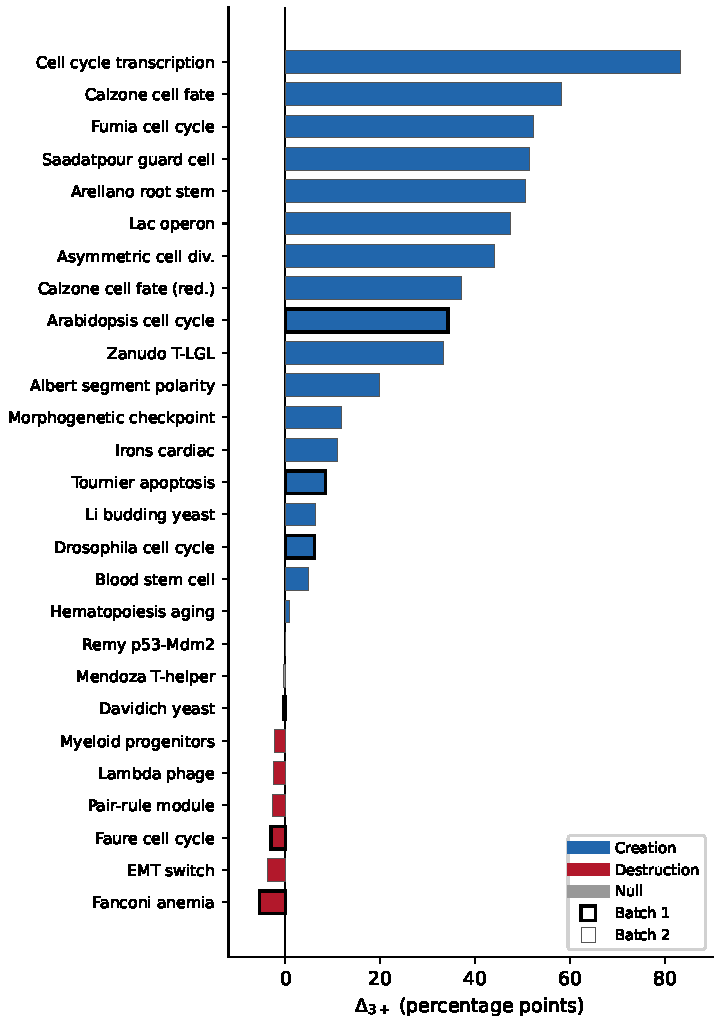
\includegraphics[width=0.65\textwidth]{fig1_delta_ranked.pdf}
\caption{Composition gap ($\Delta_{3+}$) for all 27 networks, ranked
by magnitude. Blue: creation (positive gap). Red: destruction
(negative gap). Gray: null ($|\Delta_{3+}| < 0.5$~pp). Thick
borders indicate batch~1 networks; thin borders indicate batch~2
(held-out). The gap spans three orders of magnitude, from
effectively zero to $+83$~pp.}
\label{fig:delta-ranked}
\end{figure}

\begin{longtable}{lrrrrl}
\caption{Composition gap results for 27 Boolean GRNs, sorted by
cycling fraction. $\rho$: Spearman correlation between local and
global pairwise magnitudes. $\Delta_{3+}$: global minus local
order-3+ energy (pp). Classification: creation ($> 0.5$~pp),
destruction ($< -0.5$~pp), or null.}
\label{tab:all_results} \\
\toprule
Network & $n$ & $\rho$ & $p$ & $\Delta_{3+}$ & Cycling \\
\midrule
\endfirsthead
\toprule
Network & $n$ & $\rho$ & $p$ & $\Delta_{3+}$ & Cycling \\
\midrule
\endhead
\bottomrule
\endfoot
Arellano root stem & 9 & 0.60 & $< 10^{-4}$ & $+$50.6 & 0.0\% \\
Segment polarity & 11 & 0.21 & 0.126 & $+$19.8 & 0.0\% \\
EMT switch & 12 & 0.38 & 0.002 & $-$3.8 & 0.1\% \\
Lac operon & 13 & 0.08 & 0.492 & $+$47.4 & 0.3\% \\
Cell cycle transcription & 9 & $-$0.38 & 0.021 & $+$83.3 & 0.4\% \\
Morphogenetic checkpoint & 12 & 0.40 & $< 10^{-3}$ & $+$11.9 & 0.4\% \\
Calzone cell fate (full) & 17 & $-$0.02 & 0.855 & $+$58.2 & 0.5\% \\
Mendoza T-helper$^\dagger$ & 13 & 0.21 & 0.059 & $-$0.3 & 1.7\% \\
Saadatpour guard cell & 13 & 0.07 & 0.572 & $+$51.4 & 5.7\% \\
Asymmetric cell division & 9 & $-$0.10 & 0.547 & $+$44.1 & 6.3\% \\
Myeloid progenitors & 11 & 0.51 & $< 10^{-4}$ & $-$2.3 & 6.6\% \\
Tournier apoptosis & 12 & 0.25 & 0.046 & $+$8.5 & 7.4\% \\
Irons cardiac & 15 & 0.63 & $< 10^{-12}$ & $+$10.9 & 9.3\% \\
Za\~nudo T-LGL & 12 & $-$0.19 & 0.120 & $+$33.2 & 10.3\% \\
Hematopoiesis aging & 15 & 0.63 & $< 10^{-12}$ & $+$0.9 & 10.5\% \\
Calzone cell fate (reduced) & 11 & $-$0.07 & 0.586 & $+$37.0 & 11.1\% \\
Li budding yeast & 11 & 0.53 & $< 10^{-4}$ & $+$6.3 & 12.5\% \\
Fumia cell cycle & 14 & 0.27 & 0.011 & $+$52.2 & 12.5\% \\
Remy p53-Mdm2$^\dagger$ & 10 & 0.50 & $< 10^{-3}$ & $+$0.1 & 13.4\% \\
\emph{Drosophila} cell cycle & 14 & 0.12 & 0.257 & $+$6.2 & 14.0\% \\
Lambda phage & 7 & 0.61 & 0.004 & $-$2.5 & 16.0\% \\
\emph{Arabidopsis} cell cycle & 14 & 0.21 & 0.052 & $+$34.3 & 16.4\% \\
Davidich yeast$^\dagger$ & 10 & 0.15 & 0.312 & $-$0.4 & 17.7\% \\
Pair-rule module & 11 & 0.66 & $< 10^{-7}$ & $-$2.7 & 17.8\% \\
Faure cell cycle & 10 & 0.41 & 0.005 & $-$3.0 & 19.6\% \\
Blood stem cell & 11 & 0.59 & $< 10^{-5}$ & $+$4.8 & 24.5\% \\
Fanconi anemia & 15 & 0.31 & 0.002 & $-$5.5 & 47.5\% \\
\midrule
\multicolumn{6}{l}{\footnotesize $^\dagger$Null: $|\Delta_{3+}| < 0.5$~pp.} \\
\multicolumn{6}{l}{\footnotesize 18 creation, 6 destruction, 3 null out of 27 networks.} \\
\end{longtable}


\begin{figure}[t]
\centering
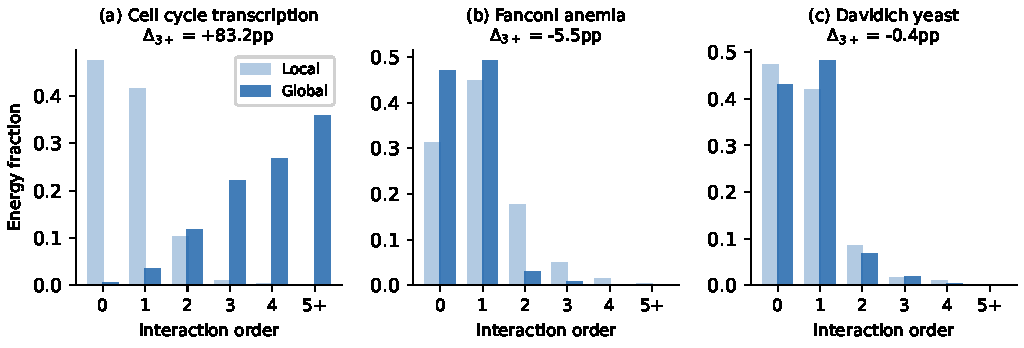
\includegraphics[width=\textwidth]{fig3_spectrum_comparison.pdf}
\caption{Local (hatched) and global (solid) energy spectra for three
representative networks. (a)~Cell-cycle transcription
($\Delta_{3+} = +83$~pp): local rules concentrate energy at orders
0--2; dynamics redistribute it into orders 3+. (b)~Fanconi anemia
($\Delta_{3+} = -5.5$~pp): dynamics compress higher-order structure.
(c)~Davidich yeast ($\Delta_{3+} = -0.4$~pp): near-identical spectra
(null case).}
\label{fig:spectrum}
\end{figure}

\subsection{Local--global correlation is positive on average but not universal}
\label{sec:rho}

The median Spearman $\rho$ between local and global pairwise
magnitudes is $0.27$ (mean $0.28$). Sixteen of 27 networks have
significant positive correlations ($p < 0.05$). In these networks,
the molecular wiring diagram provides a useful prior for predicting
which gene pairs will show knockout epistasis.

Five networks show negative $\rho$, and one of these
(cell-cycle transcription, $\rho = -0.38$, $p = 0.02$) is
statistically significant. In this network, gene pairs with strong
local Fourier interactions tend to have \emph{weaker} global knockout
epistasis. Negative correlations indicate that dynamical composition
can actively invert the interaction structure encoded in local rules.

The remaining six networks have non-significant positive
correlations, where the molecular wiring diagram carries no detectable
information about knockout epistasis.


\subsection{Limit-cycle prevalence correlates with the composition gap}
\label{sec:cycling}

Corollary~\ref{cor:decomposition} predicts that cycling fraction
should correlate with $\Delta_{3+}$. A negative association
discovered on the 6 batch-1 networks ($\rho = -0.83$) replicates in
the same direction on the 21 held-out networks ($\rho = -0.37$,
$p = 0.10$), consistent with cycle-averaging compressing
higher-order coefficients. Counterexamples exist in both directions,
so the association is suggestive rather than definitive
(Supplement~\ref{supp:cycling}).


\subsection{Structural predictions perform at chance}
\label{sec:blind-results}

SHA-frozen structural predictions on 21 held-out networks achieved
10/21 (48\%) direction accuracy, indistinguishable from chance
(Supplement~\ref{supp:blind}). A pre-registered feedback-loop-ratio
hypothesis was falsified. The composition gap is not reducible to
feedback loop counts, rule complexity, in-degree distribution, or
output-node arity; predicting it requires simulating the full
composed dynamics. More expressive structural features---such as
canalization depth or nested canalizing
structure---may improve prediction and are a natural next step.


\subsection{The composition gap survives continuous dynamics}
\label{sec:ode-results}

To test whether the composition gap is an artifact of Boolean
discretization, we converted 22 of 27 networks ($n = 7$--14) to
Hill-function ODEs (Section~\ref{sec:ode-method}) and recomputed
the coalition sweep under continuous dynamics. All 22 networks
preserve the sign of $\Delta_{3+}$ (full table in
Supplement~\ref{supp:ode-table}). Among the 19 non-null networks,
the median absolute difference between Boolean and ODE
$\Delta_{3+}$ is 1.7~pp, and magnitudes increase more
often than they decrease (13/19), suggesting that smooth Hill-function
dynamics amplify basin-boundary effects rather than compress them.
The sign persists across two-fold variation in network size
($n = 7$--14) and both creation and destruction modes, establishing
the composition gap as a property of regulatory architecture.


\subsection{Empirical fitness landscapes show higher-order creation}
\label{sec:empirical-results}

Table~\ref{tab:empirical} summarizes the Walsh decomposition of three
published fitness landscapes. In all three datasets, the composition
gap is positive: the global fitness landscape contains higher-order
epistasis that no pairwise structural or pathway interaction
predicts.

\begin{table}[t]
\centering
\caption{Composition gap in empirical fitness landscapes. Global
order-3+ energy fraction from the Walsh decomposition of measured
fitness values. Local model is additive in all cases (no structural
contacts for Weinreich; independent pathways for Hall and Franke).
Composition gap = global $E_{3+}$ since local $E_{3+} = 0$.}
\label{tab:empirical}
\begin{tabular}{llrrr}
\toprule
Dataset & Phenotype & $n$ & $E_{3+}$ (\%) & $E_{1+2}$ (\%) \\
\midrule
Weinreich TEM-1 & log(MIC) & 5 & 2.9 & 76.3 \\
Hall yeast & Haploid growth & 6 & 0.1 & 0.8 \\
Hall yeast & Mating efficiency & 6 & 4.7 & 9.5 \\
Hall yeast & Sporulation eff. & 6 & 1.2 & 4.7 \\
Franke \emph{A.~niger} & Sporulation & 8 & 11.4 & 74.0 \\
Franke \emph{A.~niger} & Spor.\ (excl.\ lethal) & 8 & 1.1 & 50.2 \\
\bottomrule
\end{tabular}
\end{table}

All three datasets show positive composition gaps. The Hall yeast
results are phenotype-dependent: the same six knockouts produce
negligible higher-order structure for growth (0.1\%) but substantial
structure for mating (4.7\%), consistent with multi-pathway coupling
during conjugation. The Franke landscape's high $E_{3+}$ (11.4\%)
drops to 1.1\% after excluding lethal genotypes, indicating floor
effects at the viability boundary. Per-dataset interpretation is in
Supplement~\ref{supp:empirical}.


%% ====================================================================
\section{Discussion}
\label{sec:discussion}
%% ====================================================================

\subsection{Creation dominance}

The most robust finding is asymmetry: dynamics create higher-order
interactions three times more often than they destroy them (18 vs.\ 6
non-null networks). This asymmetry has a natural explanation. Local
Boolean rules have bounded interaction order (at most $r_k$-way,
where $r_k \leq 6$ in these networks), while attractor-level
interactions can involve all $n$ genes through pathway composition.
The ``space'' of possible higher-order interactions grows
combinatorially with $n$ but is sparsely occupied by local rules,
so dynamics have more room to create new interactions than to
suppress existing ones.

\subsection{Implications for knockout screen design}

Where the local--global correlation is positive
(Section~\ref{sec:rho}), pathway databases provide a useful prior
for prioritizing combinatorial experiments. The composition gap
adds a more specific guide: in creation networks, dynamics generate
interactions absent from any local rule, so a screen guided by
molecular interactions alone would miss the strongest epistatic
pairs. In destruction networks, the wiring diagram over-predicts
interactions that dynamics compress. In the five networks with
negative correlations, the wiring diagram actively misleads.

\subsection{Relationship to prior work}

\citet{gjuvsland2007statistical} demonstrated that
statistical epistasis is generic in gene regulatory networks. Our
results extend this in three directions. First, the gap is quantified
order-by-order rather than detected as present/absent. Second, the
gap is signed, with creation as the dominant mode. Third, across 27
networks, the gap is not predictable from standard topological
features of the regulatory graph---a result established by the
failure of pre-registered predictions.

The global epistasis literature \citep{otwinowski2018inferring, reddy2021global} establishes that nonlinear genotype-phenotype maps
reshape interaction spectra. Our local-vs-global comparison
operationalizes this reshaping as a quantitative spectral
transformation, decomposed by interaction order.

The Walsh decomposition implementation was verified by confirming
exact recovery of analytical coefficients for all 3- and 4-input
Boolean functions with known Walsh spectra.


\subsection{Generalization and selection bias}

Three lines of evidence establish that the composition gap is not an
artifact of Boolean discretization: ODE sign preservation in 22/22
networks, phenotype-dependent higher-order structure in the Hall
yeast system, and order-3+ energy in the Weinreich and Franke
landscapes from organisms with no pairwise structural contacts or
shared pathways.

The creation dominance finding (18/6) may partly reflect selection
bias. These networks were curated from repositories that
over-represent interesting emergent behavior (multistability, complex
attractors). If dynamical complexity correlates with creation---a
plausible assumption---then the 18/6 ratio may overestimate
prevalence in gene regulatory networks generally.

An open question is whether the composition gap would persist in
random Boolean networks of matched size and connectivity. Kauffman
$NK$ ensembles or degree-preserving rewired networks would provide
a principled null: if the gap magnitude in curated networks exceeds
that of random networks with the same in-degree distribution, the
excess reflects biological regulatory structure rather than generic
nonlinear dynamics. We leave this comparison to future work.

\subsection{Limitations}

Three design choices constrain interpretation.
First, creation dominance is specific to loss-of-function (clamp-to-0)
knockout semantics. Clamp-to-1 sweeps compress gap magnitudes 6-fold
and reverse the creation/destruction ratio, because AND and OR gates
respond asymmetrically to high vs.\ low clamping.
Second, the primary analysis uses synchronous update.
Preliminary asynchronous sweeps on three networks ($n = 10$--12)
preserve the gap sign with reduced magnitude, consistent with
update-order stochasticity smoothing basin boundaries.
Third, the exhaustive $2^n$ sweep limits analysis to small
networks ($n \leq 17$). Real regulatory modules can involve
hundreds of genes; whether the composition gap scales, saturates,
or changes character at larger $n$ remains unknown.
Additional sensitivity analyses (input-node exclusion,
aggregation method) are reported in
Supplement~\ref{supp:sensitivity}.


%% ====================================================================
\section{Conclusion}
\label{sec:conclusion}
%% ====================================================================

Across 27 Boolean gene regulatory networks, we measured the complete
Walsh interaction spectrum at both the local rule and attractor
levels. Three findings emerge. First, dynamics create higher-order
epistasis three times more often than they destroy it: composition
is a generically constructive process. Second, the molecular wiring
diagram is a useful but unreliable predictor of knockout
epistasis---positive on average, negative in five networks, and at
chance for predicting the gap direction from structural features
alone. Third, limit-cycle prevalence correlates with the composition
gap ($\rho = -0.51$, $p = 0.007$), consistent with oscillatory
averaging as a compression mechanism, though counterexamples prevent
a clean separation. Hill-function ODE conversion preserves the gap
sign in 22/22 networks tested, confirming that the effect is a
property of regulatory topology rather than Boolean discretization.
The same Walsh decomposition applied to three experimental fitness
landscapes confirms that higher-order epistasis beyond pairwise
structural predictions is present in real organisms, with its
magnitude depending on which phenotype is measured.

The complete Walsh spectra, coalition value functions, and
pre-registration artifacts are available at
\textcolor{red}{[URL: Zenodo repository]}.


%% ====================================================================
\section*{Data availability}
%% ====================================================================

All data and code are available at \textcolor{red}{[URL: Zenodo DOI]}.
The repository includes: (i)~coalition value functions for all 27
networks as compressed NumPy archives; (ii)~wiring diagrams and local
Walsh spectra as JSON; (iii)~pre-registration prediction files with
SHA-256 checksums; (iv)~Walsh spectra for the Weinreich, Hall, and Franke
empirical fitness landscapes; (v)~ODE coalition value functions for
all networks with Hill-function conversion; (vi)~all analysis and
plotting scripts.
The Weinreich data originate from \citet{weinreich2006darwinian},
the Hall data from \citet{hall2010fitness} via the harmslab
repository, and the Franke data from \citet{franke2011evolutionary}.
No proprietary data or software is required.


%% ====================================================================
%% References
%% ====================================================================

\bibliographystyle{unsrtnat}
\bibliography{refs}


%% ====================================================================
\clearpage
\appendix
\renewcommand{\thesection}{S\arabic{section}}
\setcounter{section}{0}
\section*{Supplement}
%% ====================================================================


\section{Proofs}
\label{supp:proofs}

\begin{proof}[Proof of Proposition~\ref{prop:dag}]
Label the non-input nodes $1, \ldots, m$ in topological order. At
step $t$, node~$i$'s update depends only on nodes with indices
$< i$. After $d = \mathrm{depth}(\Gamma)$ synchronous steps, every
node's value is self-consistent and repeats thereafter. Because
each node's steady value is a deterministic function of the source
(input-node) values and the clamping configuration, the fixed point
is unique.
\end{proof}

\begin{proof}[Proof of Proposition~\ref{prop:creation}]
Consider four genes $x_1, x_2, x_3, y$ with rules
$h = x_1 \wedge x_2$ and $y = h \wedge x_3$, a depth-2 DAG. Each
rule has Walsh order~2. The composed function
$y(S) = (x_1 \wedge x_2) \wedge x_3$ has Walsh expansion (in
$\pm 1$ encoding)
$y = \tfrac{1}{8}(1 - z_1 - z_2 - z_3 + z_1 z_2 + z_1 z_3
+ z_2 z_3 - z_1 z_2 z_3)$,
where $z_i = 1 - 2x_i$. The $z_1 z_2 z_3$ coefficient is nonzero
at order~3, absent from every local rule.
\end{proof}


\section{Full ODE comparison table}
\label{supp:ode-table}

\begin{table}[h]
\centering
\caption{Composition gap under Boolean vs.\ Hill-function ODE
dynamics for 22 networks. Remaining 5 networks were still computing
at time of submission.}
\begin{tabular}{lrrrr}
\toprule
Network & $n$ & $\Delta_{3+}^{\mathrm{Bool}}$ & $\Delta_{3+}^{\mathrm{ODE}}$ & Sign \\
\midrule
Cell cycle transcription & 9 & $+$83.3 & $+$89.8 & preserved \\
Arellano root stem & 9 & $+$50.6 & $+$48.9 & preserved \\
Saadatpour guard cell & 13 & $+$51.4 & $+$65.4 & preserved \\
Fumia cell cycle & 14 & $+$52.2 & $+$54.8 & preserved \\
Lac operon & 13 & $+$47.4 & $+$48.9 & preserved \\
Asymmetric cell division & 9 & $+$44.1 & $+$43.4 & preserved \\
Calzone cell fate (reduced) & 11 & $+$37.0 & $+$40.1 & preserved \\
Za\~nudo T-LGL & 12 & $+$33.2 & $+$33.7 & preserved \\
Segment polarity & 11 & $+$19.8 & $+$22.7 & preserved \\
Morphogenetic checkpoint & 12 & $+$11.9 & $+$14.5 & preserved \\
Tournier apoptosis & 12 & $+$8.5 & $+$17.4 & preserved \\
Blood stem cell & 11 & $+$4.8 & $+$6.8 & preserved \\
Li budding yeast & 11 & $+$6.4 & $+$2.4 & preserved \\
\emph{Drosophila} cell cycle & 14 & $+$6.2 & $+$5.8 & preserved \\
Remy p53-Mdm2$^\dagger$ & 10 & $+$0.1 & $+$0.3 & preserved \\
EMT switch & 12 & $-$3.8 & $-$3.9 & preserved \\
Faure cell cycle & 10 & $-$3.0 & $-$2.4 & preserved \\
Pair-rule module & 11 & $-$2.7 & $-$2.8 & preserved \\
Lambda phage & 7 & $-$2.5 & $-$3.6 & preserved \\
Myeloid progenitors & 11 & $-$2.3 & $-$2.0 & preserved \\
Davidich yeast$^\dagger$ & 10 & $-$0.4 & $+$0.04 & preserved \\
Mendoza T-helper$^\dagger$ & 13 & $-$0.3 & $-$1.0 & preserved \\
\bottomrule
\multicolumn{5}{l}{\footnotesize $^\dagger$Null under Boolean dynamics ($|\Delta_{3+}| < 0.5$~pp).} \\
\end{tabular}
\end{table}


\section{Cycling fraction details}
\label{supp:cycling}

A negative association between cycling fraction and $\Delta_{3+}$
was observed post-hoc on the 6 batch-1 networks ($\rho = -0.83$,
$p = 0.04$, but post-hoc so effectively $\sim 0.10$ two-tailed).
The 21 held-out batch-2 networks show the same sign but are not
independently significant ($\rho = -0.37$, $p = 0.10$). Pooling
all 27 gives $\rho = -0.51$ ($p = 0.007$), but this includes the
discovery sample. Among non-null networks, the destruction group
has higher median cycling (16.9\%) than creation (8.3\%), but a
Mann--Whitney test is not significant ($U = 30$, $p = 0.12$).
Counterexamples: EMT switch has 0.1\% cycling but shows destruction
($-3.8$~pp); blood stem cell has 24.5\% cycling but shows creation
($+4.8$~pp). Cycling fraction does not correlate with network size
($\rho = 0.09$, $p = 0.87$).


\section{Blind prediction details}
\label{supp:blind}

\begin{table}[h]
\centering
\caption{Blind prediction accuracy. Batch~2 (21 held-out networks) is
the confirmatory test; batch~1 predictions were developed on the same
networks and are circular.}
\begin{tabular}{lccc}
\toprule
Category & Batch 2 (confirmatory) & Batch 1 (circular) \\
\midrule
Gap direction & 10/21 (48\%) & 4/6 \\
$\rho$ in predicted range & 6/21 (29\%) & 4/6 \\
fb\_ratio hypothesis & Falsified & Falsified \\
\bottomrule
\end{tabular}
\end{table}

Predicted $\rho$ ranges contained the observed value in 6/21 cases
(29\%). Batch~1 predictions (4/6) were developed on the same networks
and are therefore circular.


\section{Empirical landscape details}
\label{supp:empirical}

The Weinreich TEM-1 landscape has 2.9\% order-3+ energy, dominated
by main effects (73.1\%) as expected for mutations spread across a
263-residue protein with no pairwise structural contacts at 8~\AA.
The higher-order structure reflects long-range functional coupling
through catalytic efficiency and protein stability---the protein
analog of path composition (Proposition~\ref{prop:creation}).

The Hall yeast results are phenotype-dependent. Haploid growth is
dominated by the intercept (99.1\% order-0), with negligible
higher-order structure (0.1\%): biosynthetic knockouts have mainly
additive effects on vegetative growth. Mating efficiency has 4.7\%
order-3+ energy, comparable to many Boolean GRNs, consistent with
multi-pathway coupling through shared nutrient requirements during
conjugation.

The Franke \emph{A.~niger} landscape has the highest order-3+
fraction (11.4\%), but 70 of 256 genotypes show zero sporulation.
Excluding lethal genotypes reduces $E_{3+}$ to 1.1\%, indicating
floor effects at the viability boundary.


\section{Additional sensitivity analyses}
\label{supp:sensitivity}

\begin{itemize}
\item \textbf{Input-node exclusion.} Four networks contain
  constitutive input nodes ($f(x) = x$). Excluding these from the
  player set preserves the gap direction in all four cases (median
  magnitude change 1.0~pp).
\item \textbf{Aggregation method.} Replacing sum-aggregation with
  max-aggregation for local pairwise magnitudes
  (Eq.~\ref{eq:local-pair}) produces zero sign flips across all 27
  networks (median $\Delta\rho = -0.003$).
\end{itemize}


\section{Pre-registered predictions for extensions}
\label{supp:prereg}

Three predictions were registered before extension analyses ran
(SHA: \texttt{c66ea6...e6aef}; included in data release).

\begin{enumerate}
\item \textbf{ODE sign preservation}: predicted sign preserved under
  Hill-function conversion. Observed 22/22 preservation. ODE
  magnitudes increased more often than decreased (13/19 non-null).
  \emph{Confirmed} (sign); \emph{refuted} (magnitude direction).

\item \textbf{Weinreich TEM-1}: predicted positive gap (high
  confidence). Observed $E_{3+} = 2.9\%$. \emph{Confirmed.}

\item \textbf{Hall yeast}: predicted positive gap, small magnitude
  (medium-low confidence). Observed $E_{3+} = 0.1\%$ (haploid
  growth), $4.7\%$ (mating). \emph{Partially confirmed.}
\end{enumerate}

\end{document}
